\section*{Application: Spectra and Information in US Industry Returns}

The application uses daily value-weighted returns of the \NAssets{} Fama--French industry portfolios from \SampleStart{} to \SampleEnd{}, a total of \NDays{} trading days, taken from the CRSP 202609 vintage of the Kenneth French data library \citep{fama1997industry,french2026data}. All 49 series are complete over this period. Industry portfolios are a natural laboratory for econophysics. They are numerous enough for random matrix effects to matter at common window lengths, the economic content of their eigenvectors is easy to read, and they are diversified enough that the extreme idiosyncratic events which dominate individual stocks do not drive the spectrum. Returns are heavy tailed and heteroskedastic \citep{cont2001empirical}, so the Gaussian identities of the previous sections are benchmarks here rather than literal descriptions. Part of the purpose of the application is to see how well they survive. All statistics are computed in rolling windows of $T=250$ trading days, advanced in steps of 21 days, which gives \NWindows{} windows with aspect ratio $q=49/250=0.196$ for the correlation analysis.

\subsection*{The spectrum of industry correlations}

Figure~\ref{fig:snapshot} shows the eigenvalues of the correlation matrix estimated over calendar year 2025. Following \citet{laloux1999noise}, the Marchenko--Pastur benchmark rescales the bulk variance to $\hat\sigma^2=1-\lambda_1/N=\SnapSigma$, the variance not absorbed by the market mode, which places the upper edge at \SnapEdge. The largest eigenvalue is \SnapLambdaOne{}, so the market mode carries half of the total variance. In total, \SnapNOut{} eigenvalues exceed the rescaled edge. The bulk is more concentrated near zero than the white Marchenko--Pastur law predicts. This is the signature of free multiplicative convolution with a non-flat population spectrum, $H\boxtimes\rho_q$ in the notation of the preliminaries. Industry portfolios have heterogeneous residual variances and some near-collinear pairs, so the population residual spectrum $H$ is itself spread out, and the sample bulk inherits that spread. The white benchmark is therefore conservative for detecting outliers at the upper edge and uninformative about the lower edge.

\begin{figure}[htbp]
\centering
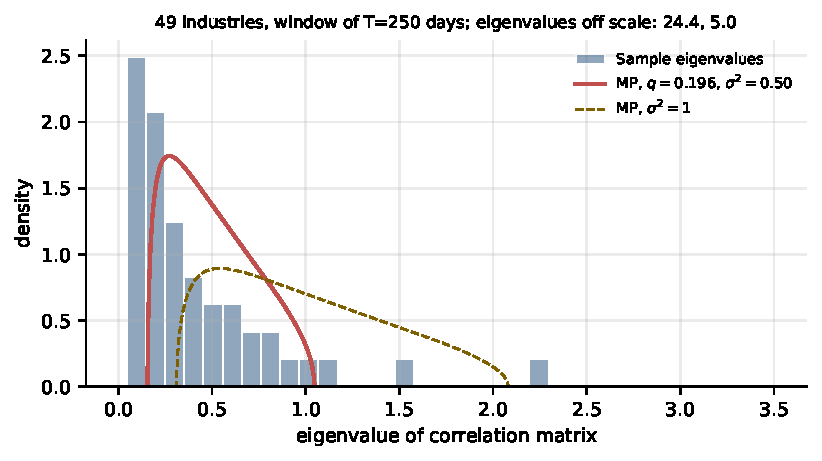
\includegraphics[width=0.8\textwidth]{figures/mp_snapshot.pdf}
\caption{Eigenvalues of the 49-industry correlation matrix over calendar year 2025 ($T=250$, $q=\SnapQ$), with the Marchenko--Pastur density rescaled by the residual variance $\hat\sigma^2=1-\lambda_1/N$ and the unscaled density for reference. The market mode ($\lambda_1=\SnapLambdaOne$) and the second eigenvalue lie off the scale of the plot.}
\label{fig:snapshot}
\end{figure}

The BBP inversion turns each outlier into a statement about reliability. Table~\ref{tab:bbp} reports, for the eight largest eigenvalues of the 2025 window, the eigenvalue scaled by $\hat\sigma^2$, the population spike $\hat\ell_k$ implied by \eqref{eq:bbp}, and the predicted squared overlap \eqref{eq:overlap} between the sample eigenvector and its population counterpart. The market mode is estimated almost perfectly. The second mode, which loads most heavily on consumer staples (soft drinks, food, household products and beer), has a predicted overlap of $0.98$. The third and fourth modes, which isolate tobacco, entertainment and defence on the one hand and precious metals, coal and mining on the other, remain well identified with overlaps of $0.93$ and $0.84$. The fifth mode is a borderline case. Its implied spike of $1.85$ lies only modestly above the threshold $1+\sqrt q=1.44$, and its predicted overlap of $0.59$ means that about forty percent of the variance of the estimated direction is noise. Its loadings mix agriculture, insurance and beverages and should not be interpreted economically. The sixth and higher eigenvalues are inside the scaled edge, and the theory predicts that their eigenvectors are uninformative. This kind of triage is the practical value of the outlier theory. It replaces the binary question of whether an eigenvalue is above the edge with a graded measure of how much the eigenvector can be trusted.

\begin{table}[htbp]
\centering
\caption{Spiked-model triage of the eight largest eigenvalues of the 2025 industry correlation matrix ($q=\SnapQ$, $\hat\sigma^2=\SnapSigma$). Scaled eigenvalues are $\lambda_k/\hat\sigma^2$ for $k\geq2$. The implied spike solves $\ell^2-(\lambda+1-q)\ell+\lambda=0$, and the predicted overlap is \eqref{eq:overlap}. A dash means the scaled eigenvalue is inside the Marchenko--Pastur bulk. Loadings are the four industries with the largest absolute eigenvector weights.}
\label{tab:bbp}
\small
\begin{tabular}{rrrrrl}
\toprule
$k$ & $\lambda_k$ & $\lambda_k/\hat\sigma^2$ & implied $\ell_k$ & predicted $|\langle u_k,v_k\rangle|^2$ & largest loadings\\
\midrule
1 & 24.38 & 24.38 & 24.18 & 0.99 & BldMt, Chems, Fin, Banks \\
2 & 5.02 & 9.98 & 9.76 & 0.98 & Soda, Food, Hshld, Beer \\
3 & 2.30 & 4.57 & 4.32 & 0.93 & Smoke, Fun, Guns, Txtls \\
4 & 1.55 & 3.08 & 2.77 & 0.84 & Gold, Coal, Mines, Rtail \\
5 & 1.14 & 2.28 & 1.85 & 0.59 & Agric, Insur, Beer, Soda \\
6 & 1.04 & 2.07 & -- & 0.00 & Guns, Coal, Oil, Drugs \\
7 & 0.90 & 1.80 & -- & 0.00 & Gold, Oil, Fun, Aero \\
8 & 0.85 & 1.69 & -- & 0.00 & Guns, Drugs, Oil, MedEq \\
\bottomrule
\end{tabular}

\end{table}

Over the full sample the picture is stable in structure and variable in intensity. Figure~\ref{fig:rolling} shows the absorption ratio $\lambda_1/N$, which is the share of variance carried by the market mode and the systemic-risk indicator of \citet{kritzman2011principal}, together with the squared overlap between the market eigenvector and the equal-weighted direction and the number of eigenvalues above the edge. Absorption averages \AbsMean{} and ranges from \AbsMin{} in the window ending in \AbsMinDate{} to \AbsMax{} in the window ending in \AbsMaxDate{}. It rises sharply around the market dislocations of 2001, 2008 and 2020 and stays elevated through the euro-area crisis. The market eigenvector never strays far from the equal-weighted direction, with a squared overlap of at least \OverlapMin{}. Its overlap tends to fall when absorption falls, as the BBP overlap formula predicts for a weaker spike. The number of outliers varies between \OutMin{} and \OutMax{}, with a median of \OutMedian{}, and is positively associated with absorption (correlation \CorrAbsOut). Crises strengthen the market mode and also separate additional sector modes from the bulk. This is consistent with the regime picture of \citet{munnix2012identifying} and with the dynamic analysis above, in which correlation shocks are spectral events that move several eigenvalues together.

\begin{figure}[htbp]
\centering
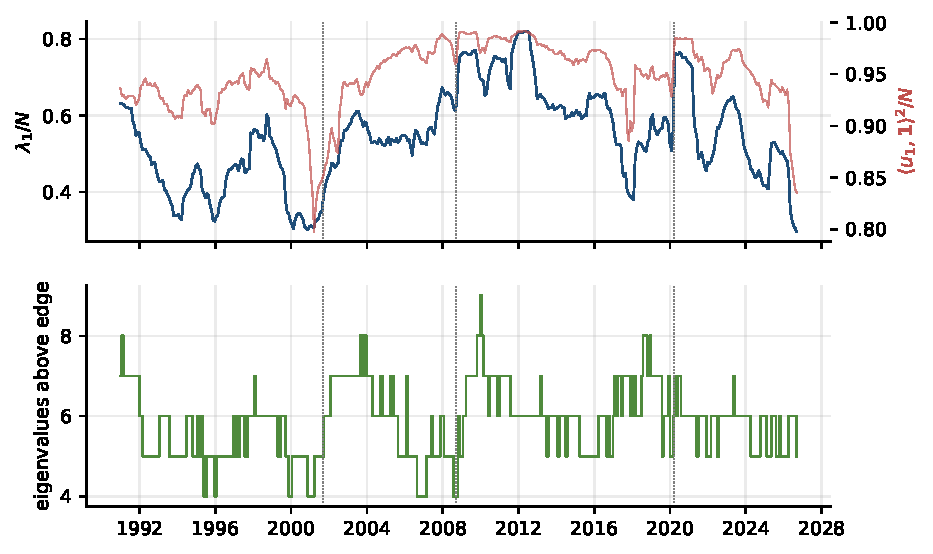
\includegraphics[width=\textwidth]{figures/rolling_spectrum.pdf}
\caption{Rolling spectral statistics, 250-day windows advanced by 21 days. Top: absorption ratio $\lambda_1/N$ (left axis) and the squared overlap of the market eigenvector with the normalised equal-weighted vector (right axis). Bottom: number of eigenvalues above the rescaled Marchenko--Pastur edge. Dotted lines mark 11 September 2001, 15 September 2008 and 16 March 2020.}
\label{fig:rolling}
\end{figure}

\subsection*{The out-of-sample cost of noise dressing}

The minimum-variance portfolio is the cleanest setting in which the cost of estimation noise can be read off directly, because it depends on the covariance matrix alone. I form global minimum-variance portfolios of the 49 industries every 21 trading days from estimation windows of $T\in\{60,120,250,500\}$ days and hold them for the following 21 days. Every estimator is evaluated on the same out-of-sample period, from the 500th trading day of the sample onward. The estimators are the sample covariance matrix, eigenvalue clipping of the correlation matrix at the rescaled Marchenko--Pastur edge \citep{laloux2000random}, linear shrinkage towards a scaled identity \citep{ledoit2004well}, and the rotationally invariant estimator \eqref{eq:rie} of \citet{bun2016rotational} with $\eta=N^{-1/2}$. Table~\ref{tab:backtest} reports realised annualised volatilities. It also reports, for the sample estimator, the ratio of realised to predicted portfolio variance next to the Gaussian benchmark $(1-q)^{-2}$ implied by \eqref{eq:gmv}.

\begin{table}[htbp]
\centering
\caption{Global minimum-variance portfolios of 49 industries, rebalanced every 21 days on a common out-of-sample period. Columns 3--6: realised annualised volatility in percent. Column 7: ratio of realised to in-sample predicted variance for the sample estimator. Column 8: its Gaussian benchmark $(1-q)^{-2}$, the product of the in-sample and out-of-sample factors in \eqref{eq:gmv}.}
\label{tab:backtest}
\small
\begin{tabular}{rrrrrrrr}
\toprule
$T$ & $q$ & Sample & Clipped & Ledoit--Wolf & RIE & $\hat R_{\rm out}/\hat R_{\rm in}$ & $(1-q)^{-2}$\\
\midrule
60 & 0.817 & 23.51 & 11.87 & 11.99 & 15.37 & 44.07 & 29.75 \\
120 & 0.408 & 13.02 & 11.84 & 11.59 & 12.06 & 3.77 & 2.86 \\
250 & 0.196 & 11.76 & 11.72 & 11.36 & 11.39 & 2.06 & 1.55 \\
500 & 0.098 & 11.59 & 11.93 & 11.46 & 11.47 & 1.63 & 1.23 \\
\midrule
\multicolumn{8}{l}{Equal weight ($1/N$): 17.93}\\
\bottomrule
\end{tabular}

\end{table}

The results follow the random matrix logic closely. With a sixty-day window ($q=0.82$), the sample estimator produces a realised volatility of \VolSampleSixty{}\%, worse than the \EWVol{}\% of the equally weighted portfolio, which is the noise-dressing failure documented by \citet{pafka2003noisy} and \citet{demiguel2009optimal}. Clipping and linear shrinkage cut that volatility in half, to \VolClipSixty{}\% and \VolLWSixty{}\%. The rotationally invariant estimator does less well at this extreme ratio (\VolRIESixty{}\%), because the sample Stieltjes transform that it relies on is poorly resolved with only 49 eigenvalues. As the window lengthens the estimators converge. At $T=250$ the spread between the best and worst is less than half a percentage point, and at $T=500$ all four lie between \VolSampleFiveHundred{}\% and \VolClipFiveHundred{}\%. At that window length clipping is slightly worse than the sample estimator, because it discards genuine sector structure below the edge. The realised-to-predicted variance ratios of the sample estimator exceed the Gaussian benchmark at every window. Examples are \RatioTwoFifty{} against \TheoryTwoFifty{} at $T=250$ and \RatioFiveHundred{} against \TheoryFiveHundred{} at $T=500$. The excess is the effect of non-stationarity and heavy tails, which inflate out-of-sample risk for every estimator. Shrinkage and the rotationally invariant estimator, which are not subject to the $(1-q)$ factors, also show realised-to-predicted ratios of about $1.5$ at $T=500$. Measured relative to that common factor, the excess of the sample estimator is about $1.23$ at $T=250$ and $1.09$ at $T=500$. This is below the Gaussian benchmark, so in these data the two sources of out-of-sample error overlap rather than compound multiplicatively.

\subsection*{Information linkage between carbon-intensive and financial industries}

The information analysis asks how much the daily returns of carbon-intensive industries reveal about the returns of financial industries. This is a reduced-form version of the transition-risk channel studied in climate finance \citep{battiston2017climate,engle2020hedging,bolton2021investors,giglio2021climate,pastor2022dissecting}. The first block contains the $p=\MIp$ industries Petroleum and Natural Gas, Coal, Utilities, Non-Metallic and Industrial Metal Mining, Steel Works, Chemicals, Transportation and Automobiles. The second contains the $r=\MIr$ industries Banking, Insurance, Real Estate and Trading. Within each 250-day window the returns are demeaned, so the relevant degrees of freedom are $n=\MIn$, and the plug-in information $\hat I$ is computed from the $12\times12$ sample covariance matrix. For this design the exact spurious information is $B_{\MIn}(\MIp,\MIr)=\MIBias$ nats, and the exact null standard deviation is $V_n^{1/2}=\MISd$. By the value-of-information theorem the same numbers, divided by $\gamma$, measure the certainty-equivalent value that an investor in the financial block would attach to observing the carbon block, were the latter available before trading. I report three variants. The first is the corrected information $\tilde I=\hat I-B_n$. The second is a placebo in which the carbon block is circularly shifted by a random offset of at least 21 days within each window, which destroys contemporaneous dependence while preserving each block's own dynamics and marginal distributions. The third is the partial information conditional on the equal-weighted market return, whose exact spurious information is $B_{n-1}(p,r)=\MIPartialBias$ nats because the regression uses one further degree of freedom.

Figure~\ref{fig:rollingmi} shows the results. The placebo is the cleanest test of the theory on real data. Its plug-in information averages \MINullPlugMean{} nats across windows against the exact prediction of \MIBias{}. Its corrected value averages \MINullCorrMean{}, and the standard deviation across windows is \MINullSd{}, against the exact $V_n^{1/2}=\MISd$. The one-sided corrected test rejects in \MINullRej\% of placebo windows at the nominal 5\% level. Despite heavy tails, volatility clustering and serial dependence, the Gaussian finite-sample theory of spurious information is accurate to the third decimal on these data. One reason is that the null law depends on the data only through the column spaces of the two blocks. It is exact whenever either column space is uniformly distributed, and in these data the departures from that condition caused by heavy tails and volatility clustering appear to be second order.

\begin{figure}[htbp]
\centering
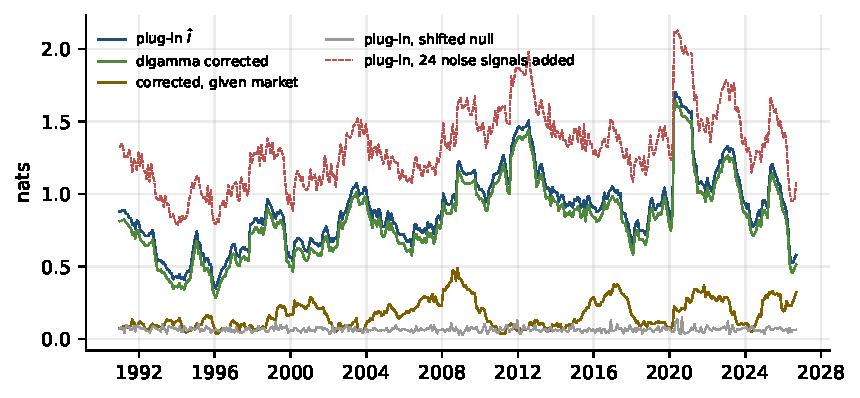
\includegraphics[width=\textwidth]{figures/rolling_mi.pdf}
\caption{Mutual information between eight carbon-intensive and four financial industries in 250-day rolling windows. Plug-in and digamma-corrected estimates, the corrected partial information given the equal-weighted market return, the plug-in estimate in a circularly shifted placebo, and the plug-in estimate after appending 24 independent Gaussian series to the financial block.}
\label{fig:rollingmi}
\end{figure}

The genuine linkage is large and highly variable. The corrected information averages \MICorrMean{} nats, compared with \MIPlugMean{} for the plug-in estimate. It is significant at the 5\% level in every window (\MIShareSig\%), ranging from \MICorrMin{} nats in \MICorrMinDate{} to \MICorrMax{} nats in \MICorrMaxDate{}, and it has a correlation of \MICorrAbs{} with the absorption ratio. Most of the information that carbon-intensive returns carry about financial returns is therefore market-wide information. Conditioning on the market removes about four fifths of it. The median share of the partial information in the total is \MIPartialShare\%. The remainder is economically and statistically distinct. The corrected partial information averages \MIPartialMean{} nats, is significant at the 5\% level in every window (\MIPartialShareSig\%), even at its minimum of \MIPartialMin{} nats in \MIPartialMinDate{}, peaks at \MIPartialMax{} nats in \MIPartialMaxDate{}, and has a correlation of only \MIPartialAbs{} with absorption. The partial linkage has its own dynamics. It rises in the run-up to and during the financial crisis, again in 2016--2017 following the commodity downturn of 2015--2016, after 2020 and in 2025--2026. None of these episodes is marked by unusually high aggregate correlation. A sector-specific informational channel between carbon-intensive industries and finance is thus present throughout the sample and is not a by-product of the market mode.

Finally, the experiment with appended noise reproduces the monotonicity proposition on real data. Adding eight independent Gaussian series to the financial block raises the average plug-in information from \MIPlugMean{} to \MIPlugNoiseEight{} nats, and adding twenty-four raises it to \MIPlugNoiseTwentyFour{}. The corresponding exact spurious information is \MIBiasNoiseEight{} and \MIBiasNoiseTwentyFour{} nats, and the predicted increments match the observed increments to the second decimal. The corrected estimates remain at \MICorrNoiseEight{} and \MICorrNoiseTwentyFour{}, indistinguishable from the \MICorrMean{} of the original design. In value terms, an evaluator who did not correct would have attributed to the padded signal set an additional $0.42/\gamma$ of certainty-equivalent value. None of that value exists.
